\documentclass[titlepage,10pt,openany]{scrbook}
%ini ukuran A6
\usepackage[papersize={107.5mm,148.5mm},twoside,bindingoffset=0.5cm,hmargin={1cm,1cm},				vmargin={1.5cm,1.5cm},footskip=0.5cm,driver=dvipdfm]{geometry}

%ini ukuran A5
%\usepackage[papersize={148.5mm,215mm},twoside,bindingoffset=0.5cm,hmargin={1cm,1cm},				vmargin={1.5cm,1.5cm},footskip=0.5cm,driver=dvipdfm]{geometry}

\usepackage[T1]{fontenc}
\usepackage{lmodern}
\usepackage{url}
\usepackage[svgnames]{xcolor}
\usepackage[utf8]{inputenc}
\usepackage{graphicx}
\usepackage{wrapfig}
\usepackage[bahasa]{babel}
\usepackage{fancyhdr}
\usepackage{pifont}
\usepackage{microtype}
\usepackage{pst-text}
\usepackage{palatino}
\usepackage{marvosym}
\usepackage{pdfpages}
\usepackage{hyphenat}
\usepackage{tikz}
\usepackage{pdfcolmk}
\usepackage{xspace}

\makeatletter
%%%% light series
%% e.g., kernel doc, section s: line 12 or thereabouts
\DeclareRobustCommand\ltseries
{\not@math@alphabet\ltseries\relax
	\fontseries\ltdefault\selectfont}
%% e.g., kernel doc, section t: line 32 or thereabouts
\newcommand{\ltdefault}{l}
%% e.g., kernel doc, section v: line 19 or thereabouts

\DeclareTextFontCommand{\textlt}{\ltseries}
% heavy(bold) series
\DeclareRobustCommand\hbseries
{\not@math@alphabet\hbseries\relax
	\fontseries\hbdefault\selectfont}
\newcommand{\hbdefault}{hb}
\DeclareTextFontCommand{\texthb}{\hbseries}
\makeatother


\renewcommand{\footrulewidth}{0.5pt}
\lhead[\fancyplain{}{\thepage}]%
      {\fancyplain{}{\rightmark}}
\rhead[\fancyplain{}{\leftmark}]%
      {\fancyplain{}{\thepage}}
\pagestyle{fancy}

\lfoot[\emph{\scriptsize Misa Peringatan 1000 hari \namaalm}]{}
\rfoot[]{\emph{\scriptsize Misa Peringatan 1000 hari \namaalm}}
\cfoot{}

\makeatletter
\newcommand{\judul}[1]{%
  {\parindent \z@ \centering 
    \interlinepenalty\@M \Large \bfseries #1\par\nobreak \vskip 20\p@ }}
\newcommand{\subjudul}[1]{%
  {\parindent \z@ 
    \interlinepenalty\@M \bfseries #1\par\nobreak \vskip 10\p@ }}
\newcommand{\lagu}[1]{%
  {\parindent \z@ 
    \interlinepenalty\@M \slshape \bfseries \normalsize \textit{#1}\par\nobreak \vskip 10\p@ }}
\newcommand{\keterangan}[1]{%
  {\parindent \z@  \slshape 
    \interlinepenalty\@M \textsl{#1}\par\nobreak  \vskip 5\p@}}

\renewenvironment{description}
               {\list{}{\labelwidth\z@ \itemindent-\leftmargin
                        \let\makelabel\descriptionlabel}}
               {\endlist}
\renewcommand*\descriptionlabel[1]{\hspace\labelsep 
                                \normalfont\bfseries #1 }


\makeatother

\newcommand{\BU}[1]{\begin{itemize} \item[U:] #1 \end{itemize}}
\newcommand{\BI}[1]{\begin{itemize} \item[I:] #1 \end{itemize}}
\newcommand{\BIU}[1]{\begin{itemize} \item[I+U:] #1 \end{itemize}}
\newcommand{\BPU}[1]{\begin{itemize} \item[P+U:] #1 \end{itemize}}
\newcommand{\BP}[1]{\begin{itemize} \item[P:] #1 \end{itemize}}
\newcommand{\inputlagu}[1]{\itshape{\input{#1}}}
\newcommand{\namaalm}{Bapak Vincentius Fererius Parlan\xspace}
\newcommand{\namaromo}{Basilius Edy Wiyanto Pr.\xspace}

\title{Misa Peringatan 1000 hari}
\author{\namaalm}
\date{oleh \\ Rm \namaromo\\10 Maret 2018}
\hyphenation{sa-u-da-ra-ku}
\hyphenation{ke-ri-ngat}
\hyphenation{je-ri-tan}
\hyphenation{hu-bung-an}
\hyphenation{me-nya-dari}
\hyphenation{Eng-kau}
\hyphenation{ke-sa-lah-an}
\hyphenation{ba-gai-ma-na}
\hyphenation{Tu-han}
\hyphenation{di-per-ca-ya-kan}
\hyphenation{men-ja-uh-kan}
\hyphenation{bu-kan-lah}
\hyphenation{per-sa-tu-kan-lah}
\hyphenation{ma-khluk}
\hyphenation{Sem-buh-kan-lah}
\hyphenation{ja-lan}
\hyphenation{mem-bu-tuh-kan}
\hyphenation{be-ri-kan-lah}
\hyphenation{me-ra-sa-kan}
\hyphenation{te-man-ilah}
\hyphenation{mem-bi-ngung-kan}
\hyphenation{di-ka-gum-i}
\hyphenation{ta-ngis-an-Mu}
\hyphenation{mi-lik-ilah}

\DeclareFixedFont{\PT}{T1}{ppl}{b}{it}{0.5in}
\DeclareFixedFont{\PTsmall}{T1}{ppl}{b}{it}{0.2in}
\DeclareFixedFont{\PTsmallest}{T1}{ppl}{b}{it}{0.15in}
\DeclareFixedFont{\PTtext}{T1}{ppl}{b}{it}{11pt}
\DeclareFixedFont{\Logo}{T1}{pbk}{m}{n}{0.3in}

\hyphenation{me-nyi-ap-kan pan-jat-kan se-jah-te-ra Par-lan o-rang bang-kit me-ma-suki me-nga-sih-ani}
\begin{document}
\thispagestyle{empty}
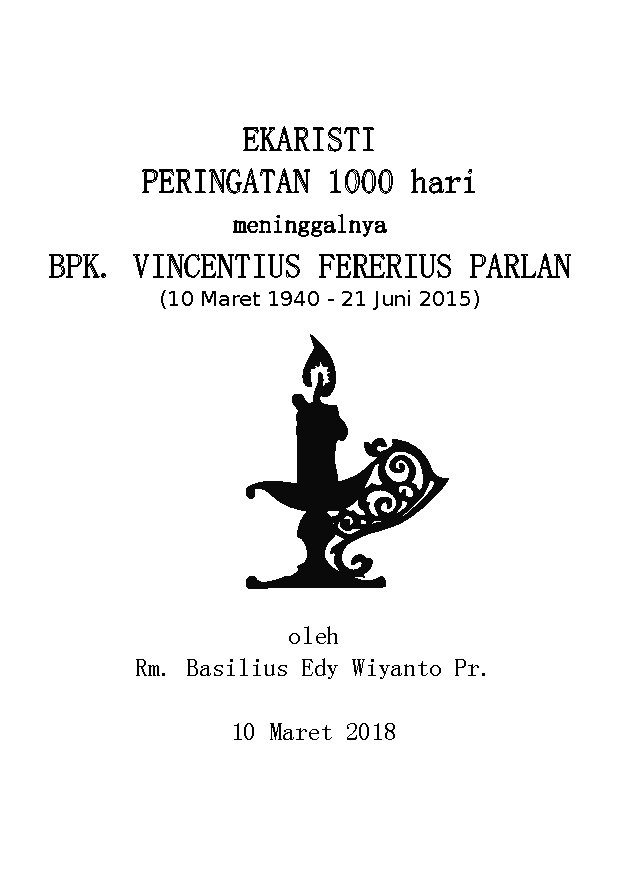
\includepdf{cover-1000-hari.pdf}

\newpage
{~}
\thispagestyle{empty}
\newpage

\section*{RITUS PEMBUKA} 

 

\lagu{Lagu Pembuka}  
\small
\begin{center}
\itshape{Bila Kau Pergi}
\end{center}
\begin{verse}
	\itshape{
Bila kau pergi\\
Ke tempat yang jauh\\
Yesus s'lalu besertamu\\
Kau dibimbingNya,\\
Kau dituntunNya,\\
S'lamat seluruh langkah hidupmu\\
{~}\\
\textbf{Refr:}\\
Biar curam g'lap\\
jalan kau tempuh\\
Hatimu sedih mengerang\\
Takkan kau penat\\
Takkan kau sesat\\
bila Yesus menyertaimu\\
{~}\\
Bila kau lelah, bila kau lesu\\
Yesus slalu besertamu\\
Kau dibujukNya, kau dihiburNya\\
Slamat kau sluruh jalanmu\\
{~}\\
Biar jauh tempat yang kau tuju\\
Biar susah mencapainya\\
Kau disambutNya kau disapaNya\\
Berbahagia kau disisiNya
}
\end{verse}
\normalsize 

\subjudul{Tanda Salib} 

\BI{Demi nama  Bapa dan Putera dan Roh Kudus}

\BU{Amin}

 

\subjudul{Salam}

\BI{Semoga kasih karunia, rahmat dan damai sejahtera dari 
Allah Bapa dan dari PuteraNya Yesus Kristus beserta 
saudara.} 

\BU{Sekarang dan selama-lamanya.}

 

\subjudul{Pengantar}

\BI{Saudara-saudari terkasih, 
	Kematian tidak memutuskan hubungan kita dengan 
	orang-orang yang sudah meninggal. Tuhan Allah tetap 
	mempersatukan kita dengan saudara kita \namaalm yang 
	dipanggil Bapa 1000 hari yang lalu. Karena kesatuan hati 
	itulah kita pada hari ini berkumpul bersama untuk 
	mendoakan arwah saudara kita. Hal ini kita lakukan 
	sebagai bentuk kasih dan kesatuan hati kita dengan 
	almarhum. Semoga doa kita semua akan mendatangkan 
	keselamatan kekal bagi saudara kita \namaalm.}


\subjudul{Tobat}

\BI{Saudara-saudari sekalian, 
	Marilah kita mempersiapkan diri, dengan memeriksa 
	batin dan hidup harian kita masing-masing. Mengingat 
	kita orang yang berdosa maka marilah kita memohon ampun dan belas kasihan dari Allah Bapa yang 
	Maharahim. Secara khusus kita juga memohonkan ampun 
	bagi dosa-dosa saudara kita \namaalm.yang dipanggil Allah 
	1000 hari yang lalu. 
	
	\textit{Hening sejenak }
	
	

Saya mengaku, \ldots \ldots
} 



\BI{Semoga Allah Bapa yang Maha Kuasa, mengasihani kita, 
mengampuni dosa kita dan mengantar kita ke dalam 
kehidupan kekal.}

\BU{Amin}

\lagu{Tuhan Kasihanilah Kami} 

\subjudul{Doa Pembuka}

\BI{Marilah berdoa\\
Allah Bapa yang mahamurah, Engkau telah menebus dosa 
kami dengan wafat dan kebangkitan Putra-Mu terkasih. 
Kasihanilah kiranya hambaMu, saudara kami \namaalm yang sudah Engkau panggil 1000 hari yang lalu. Saudara kami \namaalm percaya 
bahwa setelah kematian ada kebangkitan dan kehidupan abadi 
di surga. Semoga saudara kami ini juga Engkau perkenankan 
untuk menikmati kebahagiaan kekal abadi di surga. Demi 
Yesus Kristus, Putra-Mu, Tuhan dan pengantara kami, yang 
bersatu dengan Dikau dan Roh Kudus hidup dan berkuasa kini 
dan sepanjang masa. }

\BU{Amin}

 

\section*{LITURGI SABDA} 

\keterangan{Pembacaan dari Surat Paulus kepada umat di
Kolese (Kol 1:12-20)}

\BP{Saudara-saudari, 
	
	Marilah kita mengucap syukur dengan suka cita kepada 
	Bapa, yang melayakkan kamu untuk mendapat bagian dalam 
	apa yang ditentukan untuk orang orang kudus di dalam kerajaan 
	terang. Ia telah melepaskan kita dari kuasa kegelapan dan 
	memindahkan kita ke dalam Kerajaan Anak-Nya yang kekasih; 
	didalam Dia kita memiliki penebusan kita, yaitu pengampunan 
	dosa. Ia adalah gambar Allah yang tidak kelihatan, yang 
	sulung, lebih utama dari segala yang diciptakan, karena di 
	dalam Dialah telah diciptakan segala sesuatu, yang ada di sorga 
	dan yang ada di bumi, yang kelihatan dan yang tidak kelihatan, 
	baik singgasana, maupun kerajaan, baik pemerintah, maupun 
	penguasa; segala sesuatu diciptakan oleh Dia dan untuk Dia. Ia 
	ada terlebih dahulu dari segala sesuatu dan segala sesuatu ada 
	di dalam Dia. Ialah kepada tubuh, yaitu jemaat. Ialah kepala 
	tubuh, yaitu jemaat. Ialah yang sulung, yang pertama bangkit 
	dari antara orang mati, sehingga Ia yang lebih utama dalam 
	segala sesuatu. Karena seluruh kepenuhan Allah berkenan diam 
	di dalam Dia, dan oleh Dialah Ia memperdamaikan segala 
	sesuatu dengan diri-Nya, baik yang ada di bumi, maupun yang 
	ada di sorga, sesudah Ia mengadakan pendamaian oleh darah 
	salib Kristus.
	
	
Demikianlah Sabda Tuhan.}

\BU{Syukur kepada Allah}

\lagu{Lagu tanggapan sabda}
\scriptsize
\begin{center}
\itshape{Sabdamu Bagai Air Segar}
\end{center}

\begin{verse}
	\itshape{
SabdaMu Bapa bagai air segar, \\
sejuk dan damai saat ku dengar\\
mengalir tenang, tiada henti, \\
sumber hidup dan kasih sejati\\
{~}\\
SabdaMu Bapa bagai air segar, \\
membasahi menyuburkan bumi\\
menggugah jiwa segarkan hati,\\ 
kobarkan nurani 'tuk bersaksi\\
{~}\\
Dorong diriku ini jadi saksi kasih ilahi\\
berbekal sabdaMu wartakan janji\\
bekerja di ladangMu jadi abdi abadi\\
hari ini sampai akhir nanti\\
}
\end{verse}
\normalsize 

\subjudul{Injil}

\BI{Tuhan sertamu}

\BU{dan sertamu juga} 

\BI{Inilah Injil Yesus Kristus menurut Lukas (18:9-14)}

\BU{Dimuliakanlah Tuhan}

\BI{\textit{Pemungut cukai ini pulang ke rumahnya,  
sebagai orang yang dibenarkan Allah.}

Sekali peristiwa, 
Yesus menyatakan perumpamaan ini 
kepada beberapa orang yang menganggap dirinya benar  
dan memandang rendah semua orang lain: 
"Ada dua orang pergi ke Bait Allah untuk berdoa;  
yang satu adalah orang Farisi dan yang lain pemungut cukai. 
Orang Farisi itu berdiri dan berdoa dalam hatinya begini:  
Ya Allah, aku mengucap syukur kepada-Mu,  
karena aku tidak sama seperti semua orang lain,  
aku bukan perampok, bukan orang lalim, bukan pezinah, 
dan bukan juga seperti pemungut cukai ini. 
Aku berpuasa dua kali seminggu,  
aku memberikan sepersepuluh dari segala penghasilanku. 

Tetapi pemungut cukai itu berdiri jauh-jauh,  
bahkan ia tidak berani menengadah ke langit,  
melainkan ia memukul diri dan berkata,  
Ya Allah, kasihanilah aku orang berdosa ini. 

Aku berkata kepadamu:  
Orang ini pulang ke rumahnya  
sebagai orang yang dibenarkan Allah,  
sedang orang lain itu tidak.  
Sebab barangsiapa meninggikan diri akan direndahkan,  
dan barangsiapa merendahkan diri akan ditinggikan." }


\BI{Demikianlah Injil Tuhan}

\BU{Terpujilah Kristus}

 

\subjudul{Homili}

\subjudul{Syahadat} 

\subjudul{Doa Umat}
%---to do
\BI{Saudara-saudari, kehadiran kita bersama di sini adalah untuk mengungkapkan iman kita akan Allah sumber sukacita sejati. Marilah dengan rendah hati kita ungkapkan doa dan permohonan kita kepada Bapa:}
% % %

\BP{Bagi keselamatan saudara kita \namaalm, semoga karena kesetiaannya kepada Yesus sang Penebus 
	dan Penyelamat kita, saudara kita  \namaalm{} dihantar dan 
	dianugerahi masuk ke dalam kerajaan-Nya untuk 
	menikmati kedamaian abadi.
	
\textit{Hening sejenak \ldots\ldots} 

Marilah kita mohon :}

\BP{Ya Bapa, kedatangan Yesus Kristus di tengah-tengah kami menghadirkan tahun rahmat Tuhan kepada umat manusia. Semoga, peringatan 1000 hari meninggalnya saudara kami \namaalm ini pun, menghadirkan rahmat bagi saudara-saudari yang ditinggalkan dan kami semua yang hadir di sini.

\textit{Hening sejenak \ldots\ldots} 

Marilah kita mohon :}

\BU{Kabulkanlah doa kami ya Tuhan}


\BP{Ajarkanlah kepada kami iman, harapan, dan kasih yang sejati, agar kami mampu mengalami sukacita sejati baik di dunia ini maupun dalam persekutuan para kudus sebagaimana telah dialami oleh saudara kami \namaalm ini. 

\textit{Hening sejenak \ldots\ldots} 

Marilah kita mohon :}

\BU{Kabulkanlah doa kami ya Tuhan.}

\BP{Bantulah kami untuk meyakini bahwa hidup bukanlah berakhir di dunia ini, namun tetap berlanjut dalam kehidupan abadi bersamaMu. Semoga dalam peziarahan yang penuh tantangan ini kami tetap mampu memancarkan kegembiraan dan sukacita sejati. 

\textit{Hening sejenak \ldots\ldots} 

Marilah kita mohon :}

\BU{Kabulkanlah doa kami ya Tuhan.}

\BP{Ya Bapa, bantulah kami yang masih berjuang ini untuk meneruskan teladan dan ajaran kasih Putra-Mu, Yesus Kristus di tengah-tengah dunia yang penuh tantangan ini.

\textit{Hening sejenak \ldots\ldots} 

Marilah kita mohon :}

\BU{Kabulkanlah doa kami ya Tuhan.}

\BP{Bagi semua orang yang meninggal terutama Bapak dan Ibu Karsodinomo, Bapak dan Ibu Parjosuwito, Bapak dan Ibu Siswosudarmo, Bapak Ignatius Subiyatmo, Bapak Petrus Slamet Handoko dan Ibu Monica Soehartati, serta Bapak Atun Hudori, semoga karena kerahiman Tuhan mereka diijinkan memandang
	kemuliaan wajah Allah.
	
	\textit{Hening sejenak \ldots\ldots} 
	
	Marilah kita mohon :}

\BU{Kabulkanlah doa kami ya Tuhan.}

\BI{Bapa, kasih-Mu tiada batas. Kesabaran-Mu begitu besar. Semoga dalam pengharapan iman yang benar, kami mampu mewujudkan permohonan kami ini dalam limpahan rahmat-Mu. Dengan pengantaraan Kristus, Tuhan kami.}

\BU{Amin}

\section*{LITURGI EKARISTI}

\lagu{Lagu pengantar persembahan}
\begin{center}
\itshape{Persembahan Hidup}
\end{center}

\scriptsize
\begin{verse}
	\itshape{
Hidup kami Tuhan Engkau yang berikan,\\
Kan kami jalani demi panggilan,\\
Hidup ini memang penuh perjuangan,\\
Kadang pula penuh pergulatan.\\
{~}\\
KepadaMu hidup kami kembalikan,\\
Kedalam tanganMu sgalanya kuserahkan,\\
Suka duka tawa maupun tangisan,\\
S’moga ini jadi kidung dan pujian.\\
{~}\\
Kusembahkan hati budi diri kami,\\
Hidup mati kami dalam dunia ini.\\
Biar Kau jagai sampai akhir nanti,\\
Mengabdi Tuhan kini sampai mati.\\
{~}\\
Kami pasrah diri kepadaMu Bapa,\\
Kebebasan hidup dan cita rasa,\\
Sukma raga ini Kau jua yang punya,\\
Kesaksian kami ditengah dunia.
{~}\\
Kusembahkan hati budi diri kami,\\
Hidup mati kami dalam dunia ini.\\
Biar Kau jagai sampai akhir nanti,\\
Mengabdi Tuhan kini sampai mati.}
\end{verse}
\normalsize

\BI{Kami memuji Engkau ya Bapa, Allah semesta alam, sebab 
dari kemurahanMu kami menerima roti dan anggur yang 
kami persembahkan ini. Inilah hasil dari bumi dan usaha 
manusia yang bagi kami akan menjadi santapan rohani.}

\BU{Terpujilah Allah selama-lamanya}

\BI{Berdoalah saudara-saudara supaya persembahan kita ini 
diterima oleh Allah Bapa yang mahakuasa.}

\BU{Semoga persembahan ini diterima demi kemuliaan Tuhan 
dan keselamatan kita serta seluruh umat Allah yang kudus.}

\BI{Allah Bapa sumber kekudusan, terimalah bahan persembahan roti dananggur yang kami unjukkan untuk keselamatan hamba-Mu \namaalm. Bersama dengan keteguhan hati kami yang percaya akan belas kasihan-Mu. Kami percayakan arwah sanak-saudara kami yang telah  berpulang,  juga   hamba-Mu  \namaalm,  yang  telah 1000 hari   menghadap-Mu   ke   dalam     pangkuan   kasih-Mu   di   surga. Dengan pengantaraan Kristus, Tuhan kami.}

\BU{Amin} 

\subjudul{DOA SYUKUR AGUNG}


\subjudul{Kudus}

\subjudul{Bapa Kami}

\subjudul{Anak Domba Allah}

\subjudul{Komuni}
\newpage
\subjudul{Lagu Komuni}
\scriptsize
\begin{center}
	\itshape{nDh\`{e}r\`{e}k Gusti}
\end{center}
\begin{verse}
	\itshape{
Y\'{e}n atimu krasa ora tentrem, \\
awan bengi ora bisa merem\\
Aja nganti kow\'{e} njur salah dalan,\\
bingung pikiran lunga saparan-paran.\\
{~}\\
Rajabrana ra marakk\'{e} ayem,\\ 
pangkat mulya ra ndad\`{e}kk\'{e} tentrem\\
Ng\`{e}lingana donyan\'{e} kebak godha,\\ 
sapa l\'{e}na urip\'{e} bakal cilaka.\\
{~}\\
\textbf{Ref:}\\
Ndh\`{e}r\`{e}k Gusti Y\'{e}sus ati ayem, \\
dalan padhang pikiran dadi tenang\\
Ndh\`{e}r\`{e}k Gusti Y\'{e}sus ati tentrem, \\
sapa wong\'{e} sing ngandel lan pracaya\\
{~}\\
Ndh\`{e}r\`{e}k Gusti, atimu sing suci,\\
ndh\`{e}r\`{e}k Gusti, pasrah lan ngabekti\\
Ng\`{e}lingana Gusti nat\'{e} ngandika, \\
sing pracaya bakal\'{e} mlebu swarga
		
}
\end{verse}
\normalsize 
\scriptsize
\begin{center}
\itshape{Ave Maria}
\end{center}

\begin{verse}
\itshape{
Salam Maria penuh rahmat, Tuhan sertamu selalu\\
Terpuji di antara wanita dan terpuji buah tubuhmu.\\
{~}\\
Salam Maria penuh rahmat, Ratu surga dan dunia\\
Terpilih di antara wanita, menjadi Bunda Yesus Tuhan.
{~}\\
Ref:\\
Ave Maria 3$\times$, Bunda pengantara rahmat\\
Ave Maria 3$\times$, Bunda penuh cinta.\\
}
\end{verse}
\normalsize 

\subjudul{Doa sesudah komuni}

\BI{Marilah berdoa: 
	
	Allah Bapa yang Mahabaik, kami telah menyambut rejeki surgawi pada peringatan   seribu   hari   hamba-Mu  \namaalm   berada  dalamrumah-Mu yang abadi.  Semoga berkat Ekaristi Suci ini kami bertekun dalam iman, harapan, dan kasih, dan saudara kami \namaalm itu   menjadi   pendoa   bagi   kami   yang   masih   melanjutkan   pengabdian kami. Semoga  kami  siap  siaga  selalu  menyambut kehadiranMu  yang menyelamatkan. Dengan pengantaraan Kristus, Tuhan kami.}

\BU{Amin.}

\section*{RITUS PENUTUP}

\BI{Tuhan beserta kita}

\BU{Sekarang dan selama-lamanya}

\BI{Semoga saudara sekalian diberkati oleh Allah Yang 
Mahakuasa \Cross ~Bapa dan Putera dan Roh Kudus.}

\BU{Amin}

 

\subjudul{Pengutusan}

\BI{Saudara sekalian, Perayaan Ekaristi untuk memohon 
berkat Allah Bapa bagi arwah \namaalm telah selesai.}

\BU{Syukur kepada Allah}

\BI{Kita diutus untuk mewartakan bahwa Tuhan Yesus adalah 
jalan, kebangkitan dan hidup.}

\BU{Amin.}

 

\lagu{Lagu Penutup}

\section*{Pemberkatan Bunga Tabur, Batu Nisan, dan Burung Merpati}

\BI{Allah yang mahabaik, Engkau tahu betapa besar kasih kami kepada \namaalm, yang telah menghadap ke hadirat-Mu. 
	
\textbf{Bunga-bunga} yang akan ditaburkan di atas pusara, tempat saudara kami beristirahat selama-lamanya, menjadi tanda kasih yang harum semerbak mewangi mengiringi perjalanan hidup beliau.

\textbf{Batu nisan} akan menjadi tanda kenangan tempat beliau dibaringkan selama-lamanya.

\textbf{Burung merpati} ini melambangkan ikatan rasa, kebersamaan-persaudaraan yang tak terpisahkan, semangat perdamaian, dan kemurnian hati serta melambangkan kehadiran Roh Kudus-Mu dan kehadiran-Mu di dunia ini.

Oleh karena itu sudilah Engkau ya Bapa, mencurahkan berkat-Mu (\Cross) atas bunga-bunga, batu nisan, dan burung merpati ini. Sucikanlah dan kuduskanlah, agar segala tanda kasih ini, menjadi lambang pasrah jiwa murni sebab belas kasih-Mu, agar beliau dapat terangkat ke surga, singgasana tempat Engkau bertahta dan berada. Demi Kristus, Tuhan, dan penebus kami.
}

\BU{Amin.}

\section*{Pelepasan Burung Merpati}
\textit{Burung merpati dilepaskan melambangkan ikatan kebersa-maan-persaudaraan yang tak terpisahkan. Merpati juga melambangkan perdamaian dan penyertaan Roh Kudus atas keluarga, sanak saudara dari orang yang telah meninggal. Tindakan melepas, menandakan keikhlasan hati keluarga dalam melepaskan \namaalm yang dikasihinya untuk berdiam di rumah Bapa selama-lamanya.
{~}\\
Burung merpati dilepaskan oleh Ibu MG Waldjijah didampingi imam dan keluarga di depan gereja.} 

\begin{center}
\itshape{Sakjêgé aku ndhèrèk Gusti}
\end{center}


\small
\begin{verse}
\itshape{
Sakjêgé aku ndhèrèk Gusti\\ 
uripku tansah dibêrkahi\\
atiku ayêm têntrêm\\ 
atiku ayêm têntrêm\\ 
kabèh iku Gusti Yésus kang maringi\\
{~}\\
Sakjêgé aku ndhèrèk Gusti\\ 
uripku tansah dibêrkahi\\
atiku ayêm têntrêm\\ 
atiku ayêm têntrêm\\ 
kabèh iku Gusti Yésus kang maringi\\
{~}\\
Matur nuwun matur nuwun matur nuwun \\
Gusti Yésus kula matur nuwun\\ 
Matur nuwun matur nuwun matur nuwun \\
Gusti Yésus kula matur nuwun\\ 
}
\end{verse}
\normalsize 

\newpage
\begin{flushright}
{\Large Ucapan terima kasih}\\
\noindent Dengan penuh syukur dalam kasih Tuhan, kami mengucapkan banyak
terima kasih kepada:
\large

\textbf{Romo \namaromo}\\
yang telah berkenan memimpin perayaan ekaristi peringatan 1000 hari meninggalnya\\ \namaalm
ini.

\textbf{Koor Calista}\\
yang telah menyemarakkan perayaan ekaristi ini.

\textbf{Umat lingkungan St. Yustinus, lingkungan St. Antonius, dan lingkungan St. Theresia, para undangan, segenap keluarga, dan orang-orang terkasih}\\
yang telah berkenan hadir memberikan cinta dan doa dalam perayaan
ekaristi ini.

Semoga Tuhan memberkati dan memelihara ikatan kasih\\ di antara kita semua.

Amin.

\bigskip 

\textit{Ibu MG Waldjijah\\
dan segenap keluarga}
\end{flushright}

\end{document} 

[07:09, 5/24/2016] +62 813-2829-0020: 
Pembk hatiku percaya, antar bacaan keheningan hati, persembahan terimalah syukur kami, Kom bagaikan rusa rindukan sungaimu, penutup Asmo Dalem Maria.
[07:09, 5/24/2016] +62 813-2829-0020: Lagu misa tgl 4 Juni, ordinarium Lauda sion

Undefined control sequence. Marilah kita mohon :}